\documentclass[12pt]{article}

\usepackage[french]{babel}
\usepackage[T1]{fontenc}
\usepackage{ragged2e}
\usepackage{amsfonts}
\usepackage{systeme}
\usepackage{amsmath}
\usepackage{amssymb}
\usepackage[top=3cm, bottom=3cm, left=2.5cm, right=2.5cm]{geometry}
\usepackage{comment}
\usepackage{multicol}
\usepackage{lipsum} 
\usepackage{graphicx}
\usepackage{stmaryrd}
\usepackage{systeme}
\usepackage{wrapfig}
\usepackage{colortbl}
\usepackage{cellspace}
\usepackage{stmaryrd}
\usepackage{ntheorem}
\usepackage{lmodern}
\usepackage{mathtools}
\usepackage{ragged2e}
\usepackage{tabularx}
\usepackage{titlepic}
\usepackage{fancyhdr}
\usepackage[hypcap=true]{caption}
\usepackage{xcolor} % pour les couleurs
\usepackage[linkbordercolor=white]{hyperref} % après avoir chargé xcolor
\usepackage{systeme}
\usepackage[T1]{fontenc}
\usepackage{lmodern}
\usepackage{listings}
\usepackage{tikz}
\usepackage{mdframed}
\usepackage{xparse} % Nécessaire pour définir des environnements avec arguments optionnels
\usepackage{booktabs}  % Pour des tableaux plus jolis
\usepackage{tocloft}
\usepackage{pdfpages}
\usepackage{helvet}
\renewcommand{\familydefault}{\sfdefault}
\usepackage{setspace}



% PAGE SETTINGS

\newcolumntype{C}{>{$\displaystyle}Sc<$}
\cellspacetoplimit=5pt
\cellspacebottomlimit=5pt


% OTHERS 

% \newlength\tindent
% \setlength{\tindent}{\parindent}
% \setlength{\parindent}{0pt}
% \renewcommand{\indent}{\hspace*{\tindent}}


\usepackage{fancyvrb}
\usepackage{tikz-cd} 
\usepackage{amsmath}
\usepackage{mathrsfs}  
\usepackage{amssymb}
\usepackage{tkz-graph}
\usepackage{caption}
\usepackage{multicol}
\usepackage{listings} % Importation du package listings
\usepackage{xcolor} % Pour ajouter de la couleur

\setlength{\columnsep}{1cm} % Espace entre les colonnes


% Définition du style de l'en-tête
% \pagestyle{fancy}
\fancyhf{} % Nettoyer les en-têtes et pieds de page
\fancyfoot[C]{\thepage} % numéro de page centré en bas
\pagenumbering{arabic} % numérotation en chiffres arabes (1, 2, 3...)

% Gauche : Nom de la section
% \fancyhead[L]{\nouppercase{\leftmark}}

% Droite : Logo
% \fancyhead[R]{
\includegraphics[width=1cm]{./images/logo_jfc.png}}

% Ligne sous l'en-tête
% \renewcommand{\headrulewidth}{0.4pt}

\onehalfspacing


\begin{document}

% ==================================================================================================================================
% TITLEPAGE 

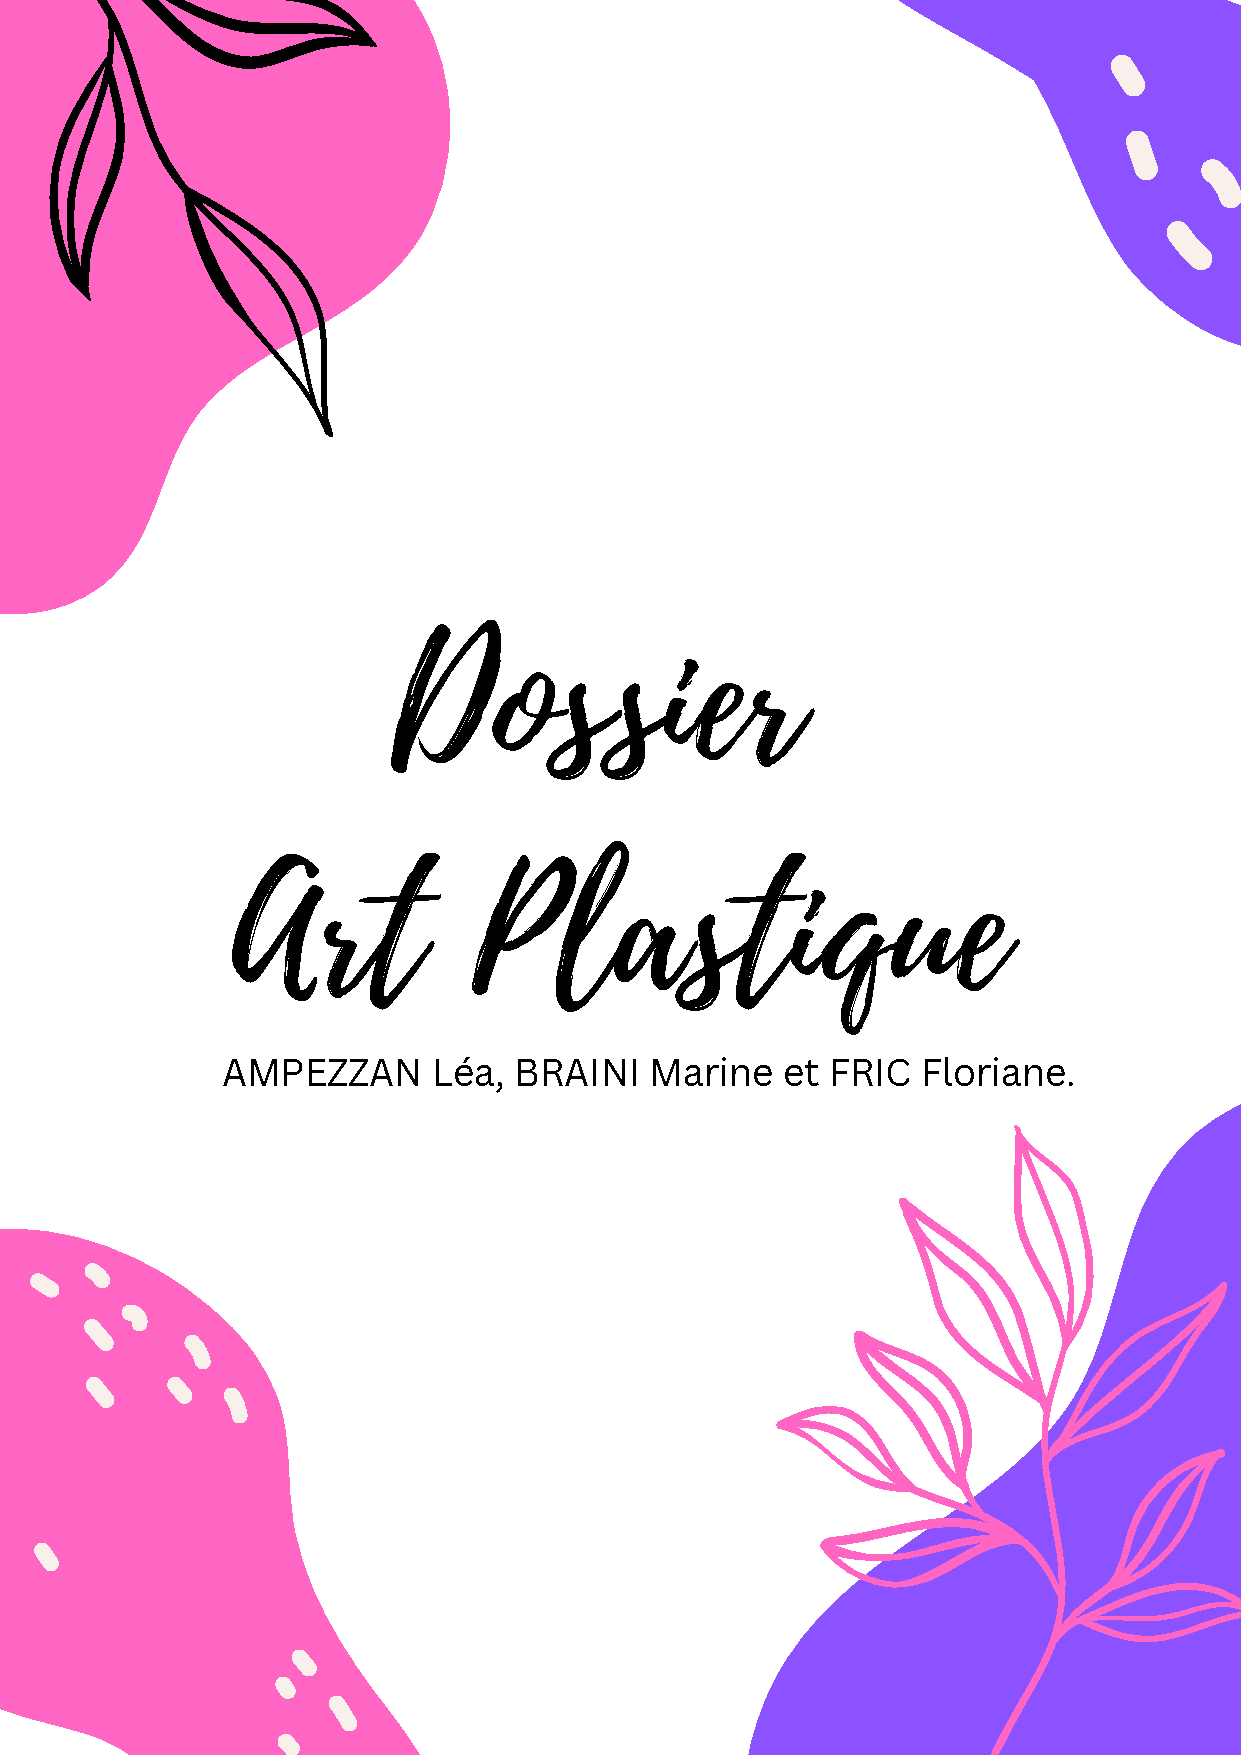
\includepdf[pages=1]{./images/titlepage.pdf}

% ==================================================================================================================================
% ANALYSE DE L'OEUVRE

\section{Analyse de l'Oeuvre}

\begin{wrapfigure}{l}{0.25\textwidth}
    \centering
    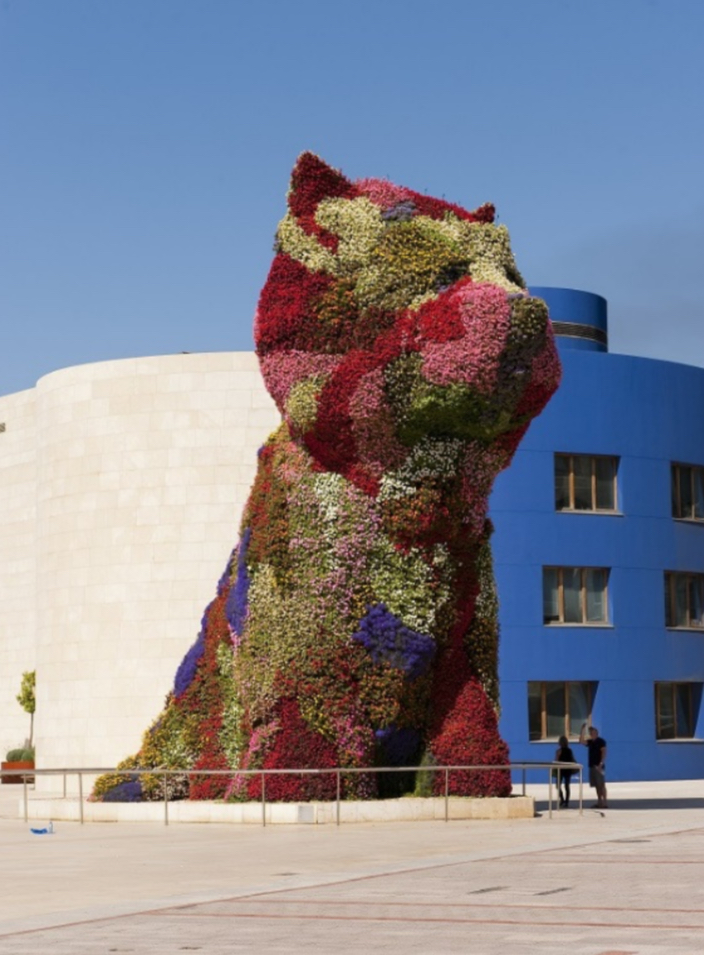
\includegraphics[width=0.2\textwidth]{./images/photo-chien.jpg}
\end{wrapfigure}

Nous observons ici la photographie d’une sculpture monumentale représentant un animal assis : un chien de race West Highland White Terrier. Le chien est dans une posture fière et droite, comme s’il veillait sur le lieu. Il tourne légèrement la tête, dans une attitude presque noble et protectrice. L’œuvre est présentée légèrement de profil, posée sur une plaque en pierre, devant un bâtiment qui a l’air plutôt moderne. Elle attire l’attention par ses dimensions hors normes et son aspect visuellement surprenant. Il s'agit de Puppy, une œuvre réalisée par l’artiste américain Jeff Koons en 1992. 

À l’origine, l’œuvre a été conçue pour être exposée devant le château baroque d’Arolsen, en Allemagne. 
Au début de sa création la sculpture mesurait 11 mètres de haut et était constituée de bois. Aujourd’hui, elle est en acier et est recouverte de fleurs naturelles mesurant 12 mètres de haut. Ici les fleurs sont dans le tond du rose, rouge. En 1997, elle est achetée par le musée Guggenheim de Bilbao, en Espagne, où elle est installée à l’entrée, comme une figure gardienne.

La taille impressionnante de Puppy et sa couverture florale donnent l’illusion d’une croissance continue, presque vivante. Cette floraison constante contribue à créer un lien fort entre la nature et la sculpture. L’agencement des fleurs crée un motif vivant, coloré, changeant au fil des saisons. L’animal a une allure imposante, comme s' il dominait l’espace.

Puppy est née dans un contexte artistique marqué par l’arrivée de nouveaux rapports à l’image, à la culture populaire et à l’espace public.

Jeff Koons a voulu capter l’attention, inspirer les artistes et transmettre des valeurs positives. Selon ses propres mots, l’œuvre exprime « la confiance et la sécurité ». Le chien se dresse fièrement devant le musée comme un gardien majestueux, solide et bienveillant. Par son apparence florale, Puppy fait également référence aux jardins classiques européens du XVIIIe siècle.

Concernant l’artiste, Jeffrey Koons est né en 1955 en Pennsylvanie. Il s’installe à New York en 1976, où il commence à bricoler ses premières œuvres. Sa première œuvre qui se démarque est The New, dans les années 1980, ce qui lui permet de se faire un nom dans le milieu artistique new-yorkais. 

Jeff Koons est un représentant du mouvement néo-pop, qui reprend les codes du pop art et précède le minimalisme. 


Le néo-pop joue sur la déformation de la réalité et la multiplication des interprétations possibles d’une œuvre en utilisant les objets du quotidien.

Koons a déclaré un jour : « Je pense que l’art vous emmène en dehors de vous-même, vous dépasse. ». Cette citation invite à réfléchir à la puissance de l’art comme expérience de dépassement de soi. C’est une forme d’évasion, mais aussi d’élévation. L’art nous sort de notre quotidien, de notre subjectivité.

Cet artiste utilise souvent des objets du quotidien dans ses créations, comme des aspirateurs exposés dans des vitrines. Cette originalité l’a démarqué. Malheureusement c’est également ce qui lui a valu plusieurs accusations et condamnations pour plagiat. 

Plus récemment, en 2024, Elon Musk a envoyé 125 sculptures miniatures de Koons sur la Lune à bord de la fusée Falcon 9. Ce geste symbolique souligne à quel point l’art de Koons a acquis une dimension universelle.

% ==================================================================================================================================
% PISTES PEDAGOGIQUES

\section{Pistes Pédagogiques}

Passons aux idées d’activités possibles pour amener l’œuvre aux élèves.

\subsection*{Activité : "Mon Puppy fleuri" (Cycle 1)}

L’activité « Mon Puppy fleuri » propose une première découverte de l’art contemporain à travers l’observation d’une œuvre et une production artistique collective et sensorielle. Inspirée de la sculpture Puppy de Jeff Koons, elle a pour objectifs principaux de stimuler le langage oral, de développer la motricité fine par le collage, de travailler les couleurs et la structuration de l’espace, tout en favorisant l’expression artistique des plus jeunes dans un cadre ludique et accessible.

L’atelier débute par un temps de langage et de découverte d’environ 10 à 15 minutes. L’enseignant montre une image de la sculpture Puppy, représentant un chiot géant recouvert de fleurs, et engage une discussion avec les enfants. À travers des questions simples – « Qu’est-ce que vous voyez ? Est-ce un vrai chien ? Pourquoi est-il plein de fleurs ? Est-ce qu’il est joyeux ? » – les élèves sont invités à s’exprimer librement. Ce moment permet d’éveiller leur curiosité et de poser les bases d’une première approche du vocabulaire artistique, en introduisant la notion de sculpture et d’ornementation florale.

Dans un second temps, l’enseignant présente l’activité de manière claire et rassurante. Il explique aux enfants qu’ils vont décorer un grand chiot tout blanc pour le rendre aussi joyeux et coloré que celui de Jeff Koons. Chaque élève reçoit une grande silhouette de chiot imprimée sur une feuille, qui servira de support à la création.

Le cœur de l’activité se déroule ensuite sous forme d’un atelier artistique de 20 à 25 minutes. Les enfants disposent de gommettes colorées (idéalement en forme de fleurs), de petits morceaux de papier de soie, de papier crépon ou de chutes de papier coloré, ainsi que de la colle en bâton ou de la colle appliquée au pinceau, selon les habitudes de la classe. Ils sont invités à coller librement ces éléments à l’intérieur de la silhouette du chiot. L’enseignant encourage les élèves à varier les couleurs et les formes, à nommer ce qu’ils utilisent (« Tu colles une fleur rose ? Tu ajoutes du jaune ici ? Bravo, ton chiot est très coloré ! »), ce qui permet de renforcer le vocabulaire descriptif tout en valorisant l’expression individuelle.

Une fois les collages terminés, un temps d’observation collective de 5 à 10 minutes permet de revenir ensemble sur les productions réalisées. Les enfants se rassemblent autour des chiots fleuris, et l’enseignant les invite à décrire ce qu’ils voient : « Est-ce que votre chiot a l’air joyeux ? Quelles couleurs avez-vous utilisées ? » Ce moment de partage valorise les réalisations de chacun tout en renforçant la cohésion du groupe et l’estime de soi.

Tout au long de cette activité d’environ 45 minutes, les enfants mobilisent des compétences essentielles pour leur développement. Ils travaillent le langage oral en nommant les couleurs et en décrivant leur action ; ils expérimentent des gestes artistiques simples (coller, organiser dans un espace défini) et développent leur motricité fine ; enfin, ils apprennent à observer une œuvre d’art, à reconnaître des formes et des couleurs, tout en vivant une première expérience de création collective inspirée par l’art contemporain.


\subsection*{Activité : "Mon chien en fleurs" (Cycle 2)}

Cette activité artistique invite les enfants à réaliser une production en lien avec les saisons à travers l’observation et la réinterprétation de l’œuvre contemporaine Puppy de Jeff Koons. L’objectif est de faire découvrir une œuvre d’art joyeuse et colorée, puis d’amener les élèves à créer leur propre "chien-fleur", en choisissant des matériaux, des textures et des couleurs évoquant leur saison préférée. Ce projet favorise à la fois la créativité, le langage oral et la sensibilité artistique des enfants.

L’activité débute par un temps de découverte de l’œuvre Puppy (environ 15 minutes). L’enseignant présente une image de la sculpture, soit projetée, soit imprimée, afin que tous les élèves puissent l’observer. Cette présentation est accompagnée d’un questionnement simple et accessible : « Que voyez-vous ? Est-ce un vrai chien ? Pourquoi y a-t-il des fleurs ? Est-ce qu’il change avec les saisons ? » L’enseignant explique ensuite que Jeff Koons a imaginé une sculpture géante et joyeuse, composée de fleurs, symbolisant la vie, la couleur et le renouveau. Ce moment de découverte permet de faire émerger chez les élèves des premières impressions et d’aborder de manière intuitive la notion de lien entre art et nature.

La phase de création (environ 40 minutes) commence par une consigne simple : chaque élève va décorer un gabarit de chien pour représenter la saison de son choix. Les enfants reçoivent une photocopie d’un gabarit de chien vierge, qu’ils vont personnaliser. Pour cela, une grande variété de matériaux à coller est mise à leur disposition : papiers colorés, morceaux de tissus, coton, etc., ainsi que des ciseaux, colle, feutres et crayons de couleur. Le matériel est organisé de manière à évoquer les différentes saisons, permettant aux élèves de faire des choix en lien avec leur univers sensoriel : des couleurs chaudes pour l’automne, des matières douces pour l’hiver, des fleurs et du vert pour le printemps, des teintes éclatantes pour l’été. Ils sont encouragés à ajouter des textures pour représenter des éléments naturels comme les fleurs, le feuillage, la neige ou le soleil. Une grande silhouette du chiot est affichée au tableau ou au centre de la salle, pour servir de modèle visible et inspirant.

Les élèves qui terminent plus tôt peuvent enrichir leur production en dessinant des détails autour du chiot : ciel, papillons, paysages, maisons, etc. Cette activité permet ainsi à chacun de s’exprimer librement tout en s’inspirant d’un cadre artistique commun.

Enfin, un temps de mise en commun (10 à 15 minutes) est organisé en regroupement. Les élèves sont invités à présenter leur "chien-fleur", à décrire leur création et à partager ce qu’ils ont aimé faire. Ils peuvent également faire le lien entre leur travail et l’œuvre de Jeff Koons, en exprimant ce qui, selon eux, rappelle Puppy dans leur propre réalisation. Ce moment d’échange favorise le développement du langage oral, la prise de parole en groupe et la valorisation des productions de chacun.

Tout au long de cette activité, les élèves mobilisent plusieurs compétences : en arts plastiques, ils réalisent une production en surface en lien avec une intention simple (évoquer une saison) ; en langage oral, ils apprennent à décrire une image ou une œuvre ; en questionnant le monde, ils observent le vivant, en faisant des liens entre la nature, les saisons et les représentations artistiques. L’activité propose ainsi une entrée ludique et sensible dans la découverte de l’art contemporain, tout en développant l’imaginaire et la créativité des élèves à partir de matériaux simples et accessibles.

\subsection*{Activité : "Puppy" géant en maquette végétale (Cycle 3)}

Cette activité artistique propose aux élèves de découvrir la sculpture et la notion de volume en s’inspirant de l’œuvre contemporaine Puppy de Jeff Koons. Elle vise à sensibiliser les élèves à la démarche artistique en les invitant à observer, comprendre et s’approprier les codes de l’art contemporain à travers la création collective d’une sculpture végétale. L’objectif est de favoriser la créativité, l’expression personnelle et le travail en équipe tout en explorant l’utilisation de matériaux naturels dans une pratique artistique.

L’activité commence par une phase d’introduction durant laquelle l’enseignant présente l’œuvre Puppy, une imposante sculpture de chiot entièrement recouverte de fleurs, réalisée par Jeff Koons. Cette présentation est accompagnée de questions visant à susciter la réflexion chez les élèves : qu’est-ce qu’une sculpture végétale ? Pourquoi utiliser des plantes pour créer une œuvre d’art ? Qu’est-ce qu’un Land Artist ? Ces interrogations permettront d’ouvrir le débat et de poser les premières bases de la compréhension de l’art contemporain. Des exemples visuels d’autres sculptures végétales viendront enrichir cette phase d’observation.

Ensuite, la classe est divisée en petits groupes de deux ou trois élèves. Chaque groupe est invité à choisir un animal qu’il représente sous la forme d’une sculpture végétale. Pour cela, les élèves utilisent des matériaux naturels tels que des feuilles, branches, fleurs, mousse ou pierres, collectés à l’avance ou apportés pour l’occasion. Ils disposent également de supports de base comme du carton, du bois ou des socles, sur lesquels ils construiront leur œuvre. Pour assembler les éléments, ils utilisent de la colle, du fil de fer, des ciseaux, et peuvent réaliser au préalable des croquis préparatoires à l’aide de papier et de crayons. Ils sont encouragés à expérimenter différentes techniques d’assemblage, comme la superposition, l’enroulement ou encore le collage, afin de donner forme à leur animal. Des croquis préparatoires peuvent être réalisés pour guider la construction.

Une fois les sculptures terminées, chaque groupe présente son œuvre à l’ensemble de la classe. Cette étape de restitution permet à chaque élève de verbaliser son processus de création, d’expliquer les choix esthétiques réalisés et de partager son ressenti. Une exposition en classe peut être organisée pour valoriser le travail accompli.

Au fil de cette séance d’environ 1h30, les élèves développent plusieurs compétences : la collaboration et le travail en équipe, la création artistique, l’expression personnelle ainsi qu’une meilleure compréhension de l’usage des matériaux dans l’art. L’activité constitue une immersion ludique dans le monde de la sculpture végétale, tout en favorisant l’exploration d’une pratique artistique accessible et stimulante. Elle permet également d’aborder l’art contemporain sous un angle concret et participatif, en renforçant le lien entre nature, créativité et expression collective.

% ==================================================================================================================================
% CONCLUSION

\section{Conclusion}

Pour conclure, ce dossier a permis d’explorer l’œuvre monumentale Puppy de Jeff Koons sous différents angles : artistique, historique et pédagogique. À travers l’analyse de la sculpture et la mise en œuvre d’activités adaptées aux cycles 1, 2 et 3, il s’agit de sensibiliser les élèves à l’art contemporain tout en développant leur créativité, leur expression personnelle et leur regard sur le monde. Les propositions pédagogiques présentées visent ainsi à rendre l’art accessible, vivant et porteur de sens dès le plus jeune âge.


\end{document}
